\chapter{Materials and Methods}
    Research and experiments require some materials. Methods for different techniques, metrics and calculations are also required to be explained. In this chapter, we have described the materials used in our research and experiment. Also the methods for training and evaluation process have been discussed here.
    
    \section{Data and Dataset}
        Data, plural form of datum, are individual units of information. It describes single quality of quantity of some object or phenomenon.
        
        A dataset is a collection of data. It may contain various kinds of data such as image, video, audio, text etc. It comprises various categories of data and types---
        \begin{enumerate}
         \item Training Data
         \item Validation Data
         \item Test Data
        \end{enumerate}
        Each of these categories is used for different purposes. Now we are going to describe the uses and purposes of the dataset categories.
        
        \subsection{Training Data}
            A category of dataset which contains data to be used to train-up the model. This may be supervised or unsupervised. In case of supervised learning, training data is annotated and actual class or label is given. The model consumes these data and tries to make prediction on them. If any wrong prediction is performed the parameters of the model e.g. bias, weight etc. are updated accordingly based on the loss or displacement from the actual one.
            
            In case of unsupervised learning, the training data may be annotated but the actual class or label is not shown to the model.
            
        \subsection{Validation Data}
            The category of data which is used to measure the validity of the novel trained model. A model may perform well when it is fed with the data used to train-up it. But it may happen that the model performance degrades for the novel data which was not shown to the model during training process. Therefore, a dataset distinct with respect to the training data is required for the proper evaluation of the model.
            
            The validation dataset is also annotated and its class-labels or actual outputs are given. If the model-performance is satisfactory on the validation data, it is assumed that it will perform well for other novel data that the model had never seen.
            
        \subsection{Test Data}
            It is a category of dataset that is used to test the performance of the model proposed. Sometimes, validation data and test data both are considered same and used interchangeably. The feeding process of test data to a model is same as the validation data.
            
            In our research, we have skipped the test dataset, rather we have used the same validation dataset for both validation and testing purposes.
            
    \section{Machine Learning (ML)}
        Machine learning is a branch of artificial intelligence where machines can learn an apply the acquired knowledge. It gives computer to learn without being programmed explicitly.It has evolved from the study of pattern recognition and computational learning theory in \acrfull{ai}. It explores the study and construction of algorithms which can be used to learn from and make predictions on data. Such algorithms can overcome strictly static program instruction by making data-driven predictions and decisions through the building of models from input.
        
        \acrshort{ml} tasks are basically classified into three broad categories depending on the learning mechanism and ``signal'' or ``feedback'' available to the system for learning---
        \begin{itemize}
         \item Supervised Learning
         \item Unsupervised Learning
         \item Reinforcement Learning
        \end{itemize}
        
        \begin{figure}[h]
            \centering
            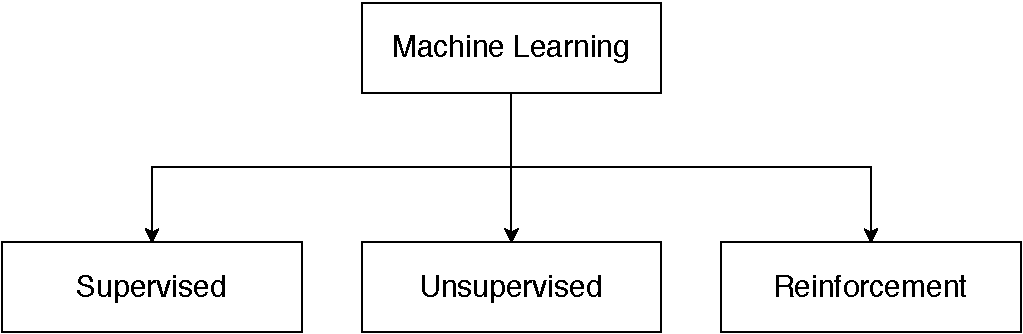
\includegraphics[width=\textwidth]{ml-types}
            \caption{Categories of Machine Learning}
            \label{fig:ml_types}
        \end{figure} 
        
        \subsection{Supervised Learning}
            This is like generating a rule that maps inputs to outputs. The computer is given example inputs along with their desired outputs. Because of the actual outputs against the inputs are exposed, more precisely, actual outputs are ``supervised'' at the learning phase by the candidate model, this approach is named as ``Supervised Learning''.
        
            \begin{figure}[h]
                \centering
                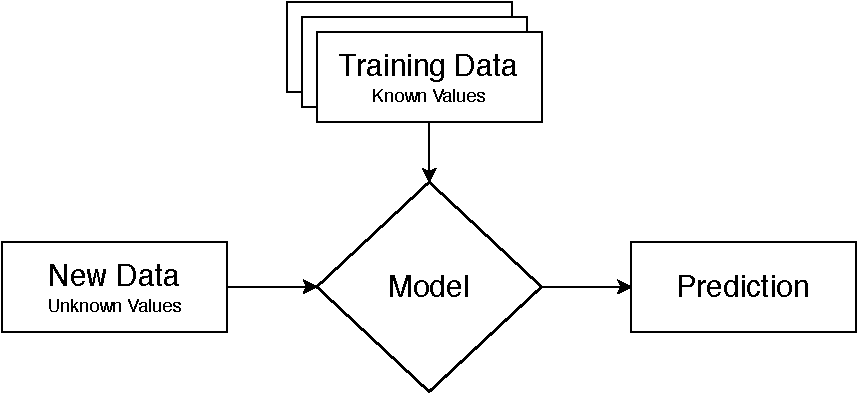
\includegraphics[width=\textwidth]{supervised-ml}
                \caption{Block Diagram of Supervised Learning}
                \label{fig:supervised_ml}
            \end{figure} 
            
            
        \subsection{Unsupervised Learning}
            This type of machine learning is like discovering hidden patterns in data. It is also known as feature learning. No desired output is exposed to the candidate model. Even the possible outputs or their number may be may be unknown or countably infinite. The learning model finds and creates the features and structures of its inputs. It may be a goal in itself or a mean towards an end.
            
        \subsection{Reinforcement Learning}
            The candidate model is provided feedback in terms of reward and punishment in this learning method. The model interacts with a dynamic environment where it is ``forced'' to perform some actions for example driving a vehicle or playing against an opponent. The action it performs targets a certain goal. If the goal is reached the model gets ``reward'' otherwise it is ``punished''. Thus the model learns through mistakes it performs.
            
            \vspace{5mm}
            There are many (possibly a lot of) machine learning algorithms and techniques. Among them, we have chosen \acrfull{cnn} approach to be used in our research and experiments.            
        
    \section{Convolutional Neural Network}
        
        \begin{figure}[h]
            \centering
            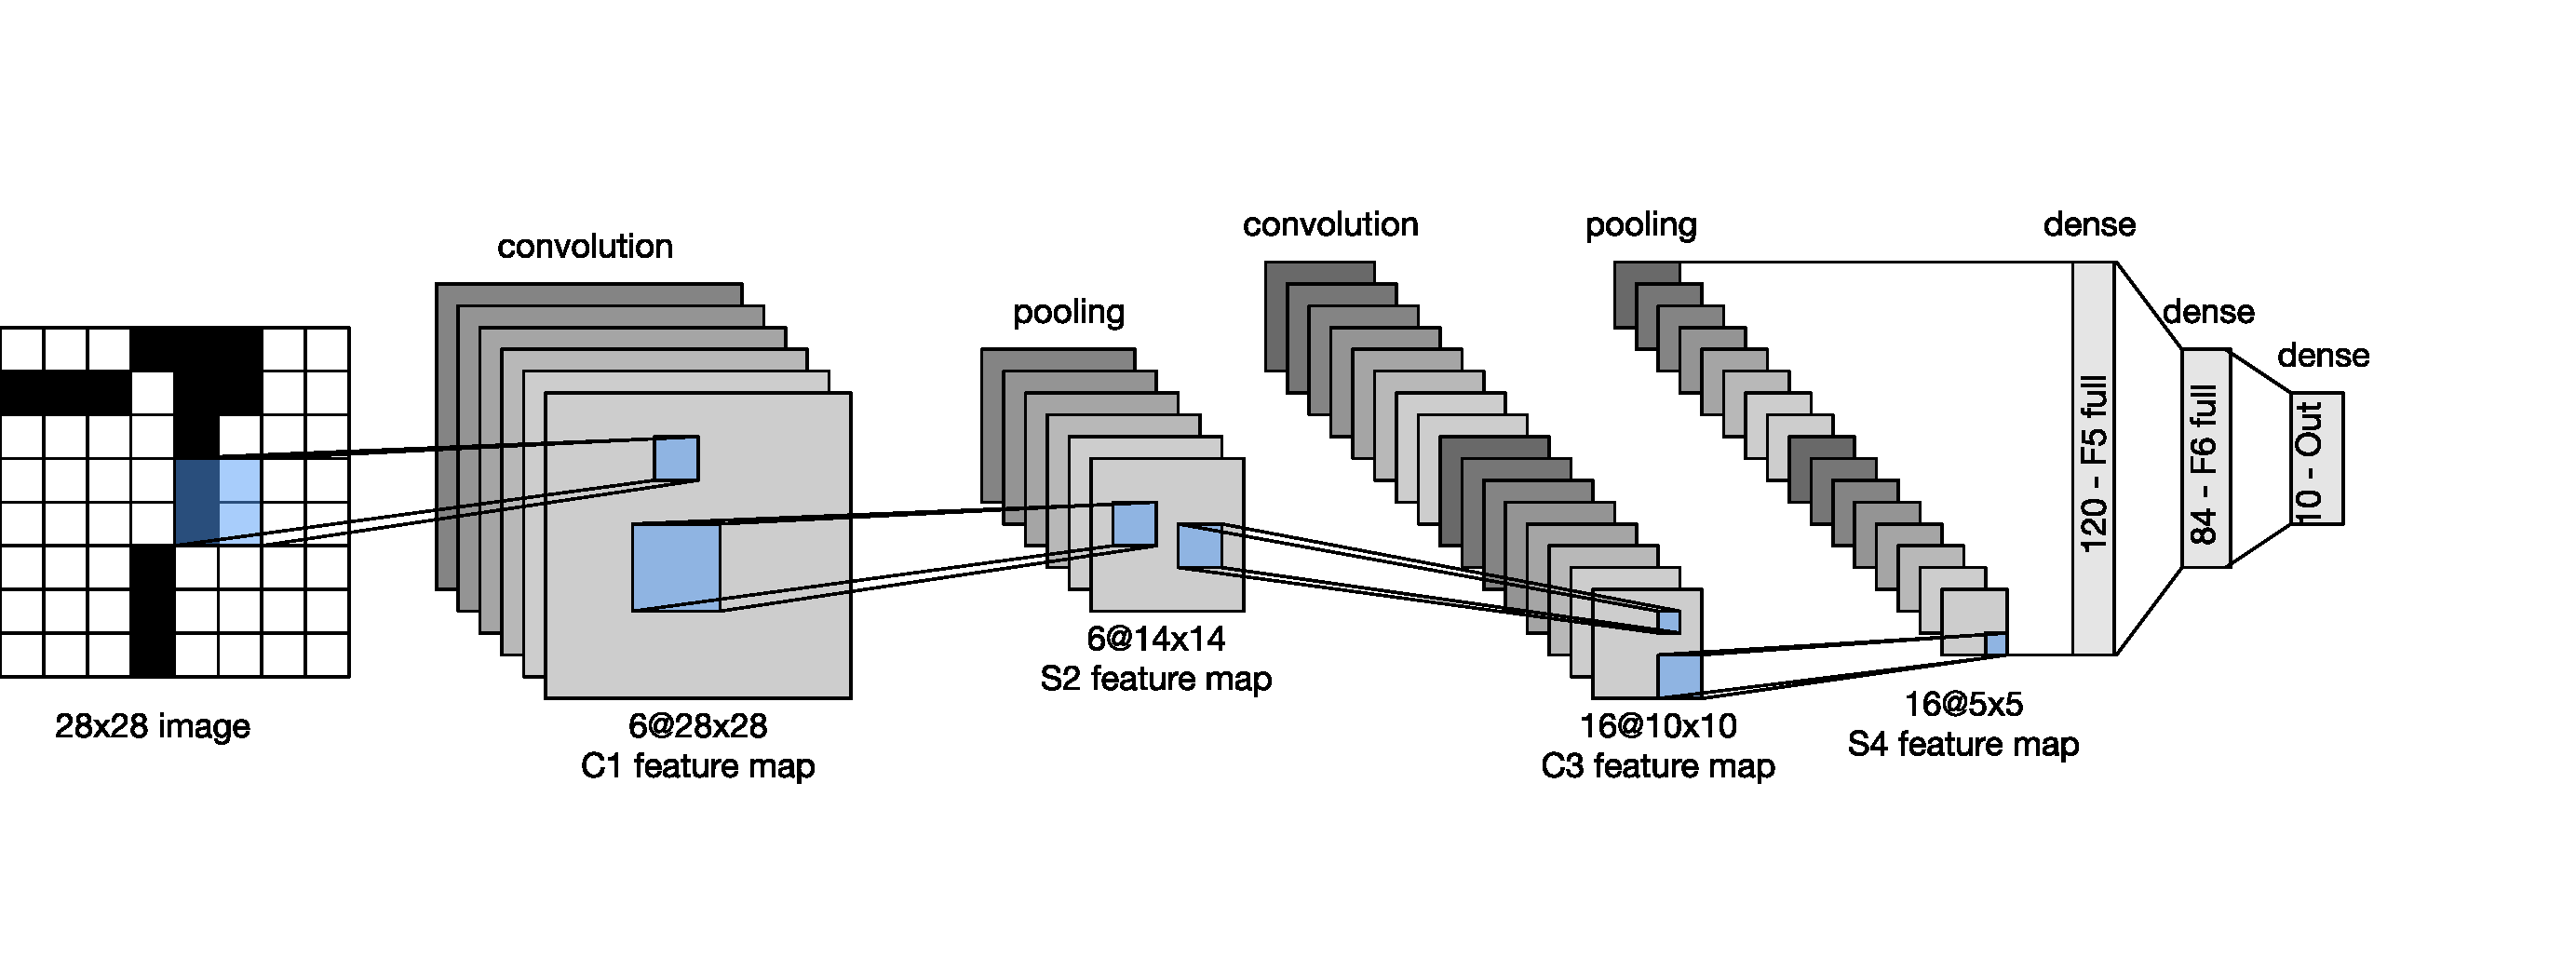
\includegraphics[width=\textwidth]{convnet}
            \caption{An Illustration of Convolutional Neural Network}
            \label{fig:convnet}
        \end{figure}   
    
        \subsection{Input Layer}
            The input layer is nothing but a door to feed the input to the network model. The shape of the input layer must be similar to the shape of input data. Therefore, if we want to pass an image with a shape of $(300\times 300\times 3)$ then the input layer must have minimum of (or exactly) $300\times 300\times 3 = 270,000$ neurons.
        
        \subsection{Convolution Layer}
            The actual feature extraction is done in this layer. ``convolution'' of the input data with the filters specified for each features is performed. A particular filter is responsible for a particular feature capturing. This process of convolution makes a drastic change in the computation of huge calculations required for traditional fully connected neural network approach. Because, convolution is performed against the filters and they are of small sizes. A portion of the input image is passed to a neuron rather than the whole. 
            \begin{figure}[h]
                \centering
                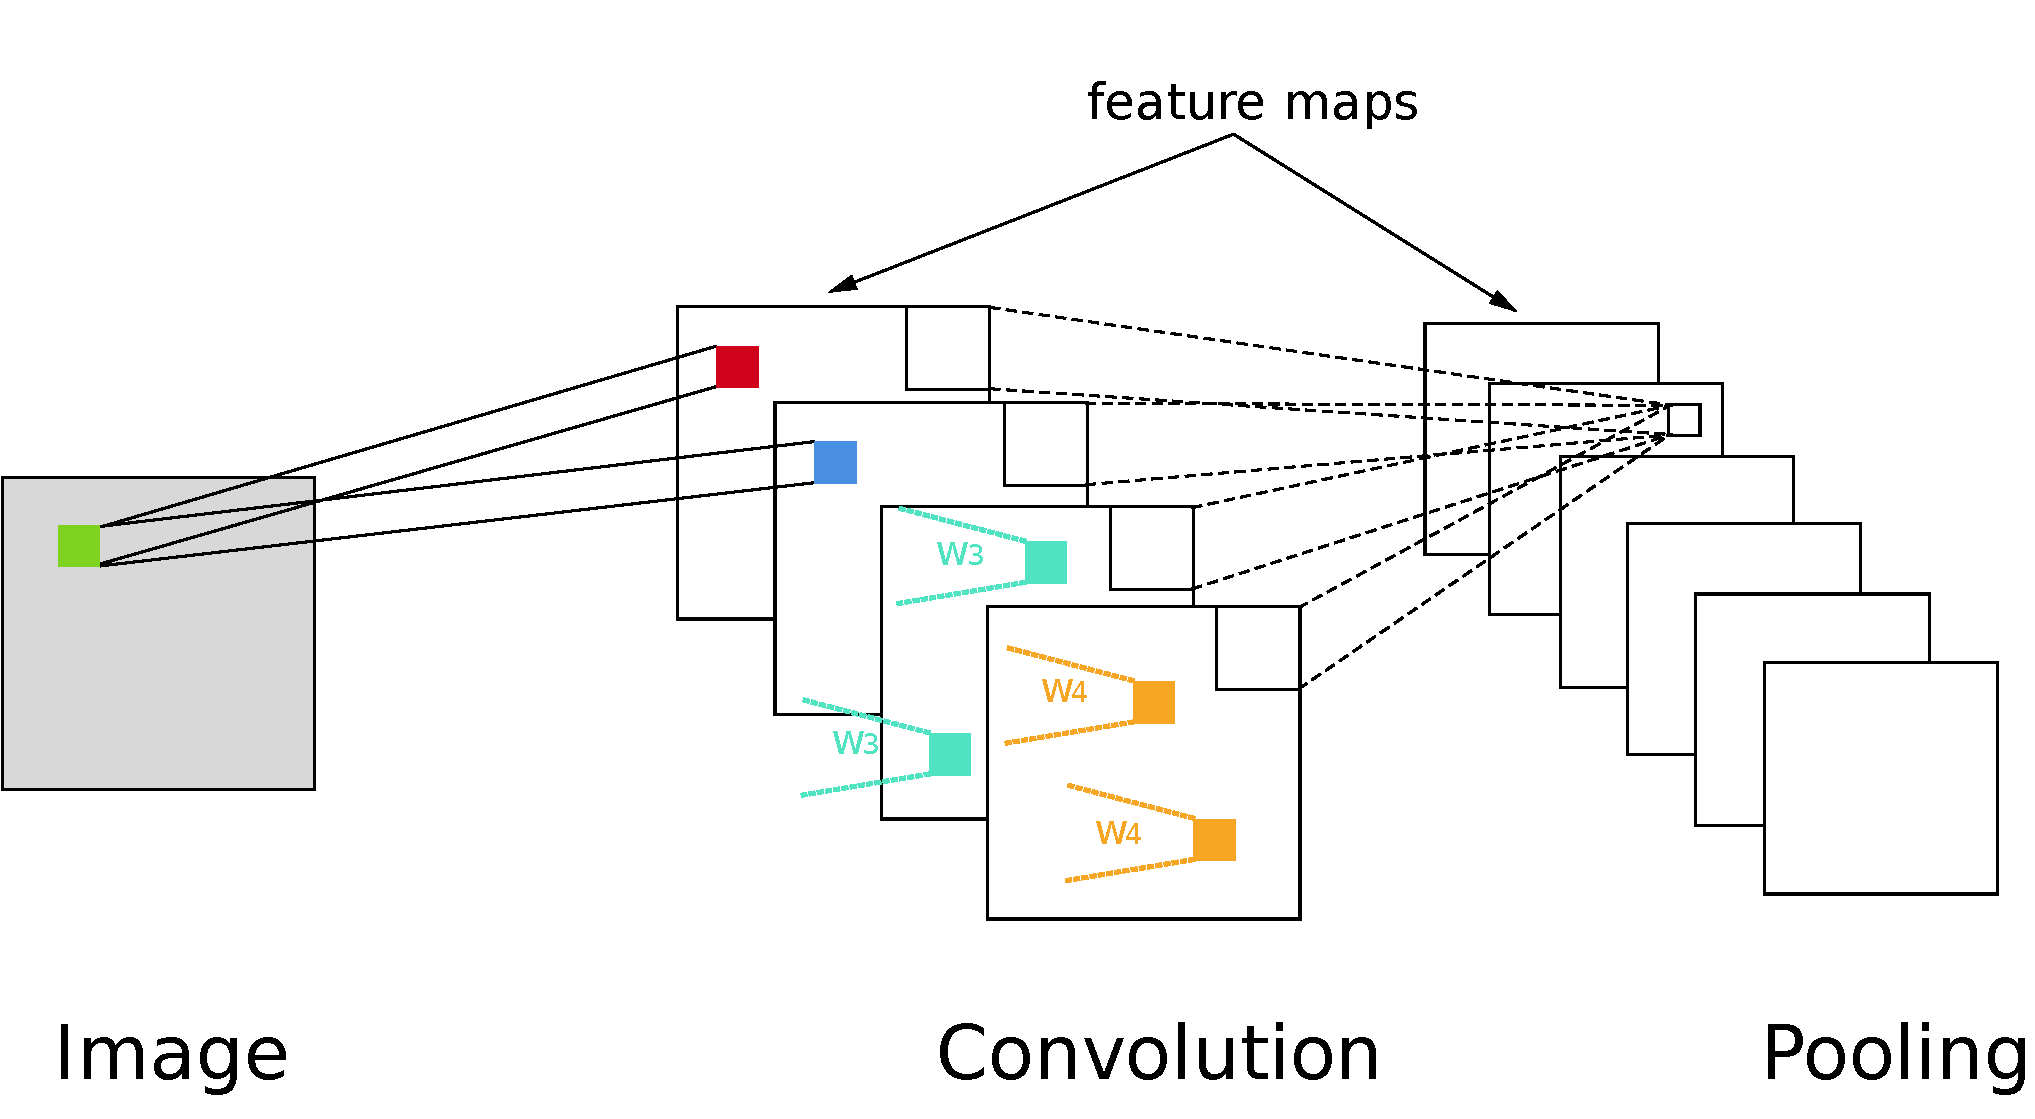
\includegraphics[width=\textwidth]{conv-layer}
                \caption{Working of a Convolution Layer}
                \label{fig:conv_layer}
            \end{figure}
    
        \subsection{ReLU Layer}
            \gls{relu} is an abbreviation of Rectified Linear Unit. It is an activation function for the neurons of a neural network model. This layer activates the required neurons who have values greater than zero. It silently converts the negative values to zero. But the neurons having non-zero non-negative values will be activated and will be linearly powered up according to their values.
    
        \subsection{Pooling Layer}
            Pooling layer is used to down-sample the large output of convolution layer for efficient computation purpose. Images may have thousands of millions of features. Filters are used to catch these features. Therefore, to get all the features from an image, we need, in theory, millions of filters; but it is almost impossible to cope with this huge number of computations using modern computers. Although for this limitation, a significant amount of filters are used for feature capturing. But, these filters cause a large shape of output from the convolution layer. So, pooling function is used to down-sample the convolutional output.      
            \begin{figure}[h]
                \centering
                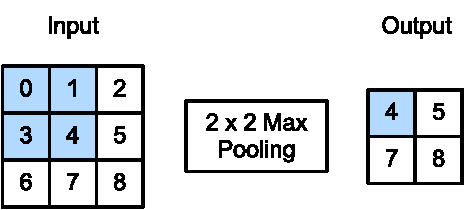
\includegraphics[width=\textwidth]{pooling}
                \caption{Working of a Pooling Layer}
                \label{fig:pooling}
            \end{figure}
    
        \subsection{Fully Connected Layer}
            This is actually the same as traditional \acrfull{ann}. Each of the layers inside and after it is of uni-dimensional. The actual prediction is done in this layer. Learning a neural network model for classification, detection, prediction actually refers to training in these layers.
            
            Usually a softmax function is applied to the last layer of this type, also known as the output layer, to perform non-maximum suppression. Thus a single class can be predicted choosing the maximum from the probabilities of all the different classes.
            \begin{figure}[h]
                \centering
                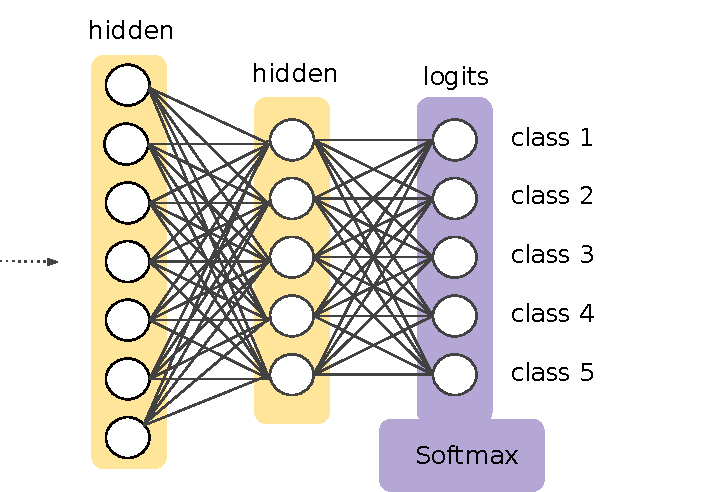
\includegraphics[width=\textwidth]{fc-layer}
                \caption{Example of Fully Connected Layer}
                \label{fig:fc-layer}
            \end{figure}
        
    %%%%%%%%% BEG: Methodology %%%%%%%%%%
    \clearpage
    
    \section{Dataset Acquisition}
        The dataset we used to train our model was a dataset which contains images as data. Those images contains various number of potholes in it. Although for training and validation purposes static images were used to constitute the dataset, our final model is capable of working with video data. It extracts the frames from the input video and treats them as images. Then it runs inference on these video frames to detect potholes.
        
        \subsection{Scrapping Web for Images}
            Google Image Search is a perfect tool for finding heterogeneous images. It displays images found in different websites, blogs, videos, articles, journals, online-newspapers etc. Therefore, we took this chance for dataset collection. Although some of these images claims copyrights, we filtered out the results to form the final dataset.
            
            It is worth mentioning that we have taken some of our dataset from Kaggle, where the dataset provider also used web-scraping to make-up the dataset.
            
        \subsection{Capturing Images of Damaged Roads}
            Our dataset contains a portion of images captured by us with a digital smart-phone camera. We have traveled the damaged roads in our campus and looked for locations having pothole. When we found a significant pothole on the pavement, we captured it.
            
            Our captured images were in \acrshort{hd} quality so that enough features can be extracted from it for training.
            
        \subsection{Image Annotation}
            After collecting enough images having potholes from various sources, it is required to select the regions of interest. The whole image is not a pothole, rather, a portion of image contains potholes. Therefore, those regions need to be explicitly exposed to the model for training. There are plenty of tools to annotate images, videos, audio, text etc. Among them, we have used \gls{labelimg}. It can be used to produce both Pascal \acrfull{voc} and Yolo format annotations. We instructed it to produce Pascal \acrshort{voc} format annotation which is an \acrshort{xml} file format. A single \acrshort{xml} file contains annotation of a single image. Samples of these formats are given in Appendix \ref{app:af_voc} and Appendix \ref{app:af_yolo}.
            
    \section{Feature Extraction}
        Machine learning approaches learns something called ``feature'' and finds these on novel data to predict what it is. To train the machine with images, we need a method for extracting the features contained in the regions of interest of the images and feed these feature to the model. Also for inference case, the features must be extracted based on which the prediction is performed.
        
        We have used an existing deep neural network model which was developed for the mobile and embedded devices keeping in mind their computing capabilities. The name of our feature extractor is \gls{mobilenet}, a deep convolutional neural network model proposed and developed by Google Researchers.
        
        \begin{figure}[h]
            \centering
            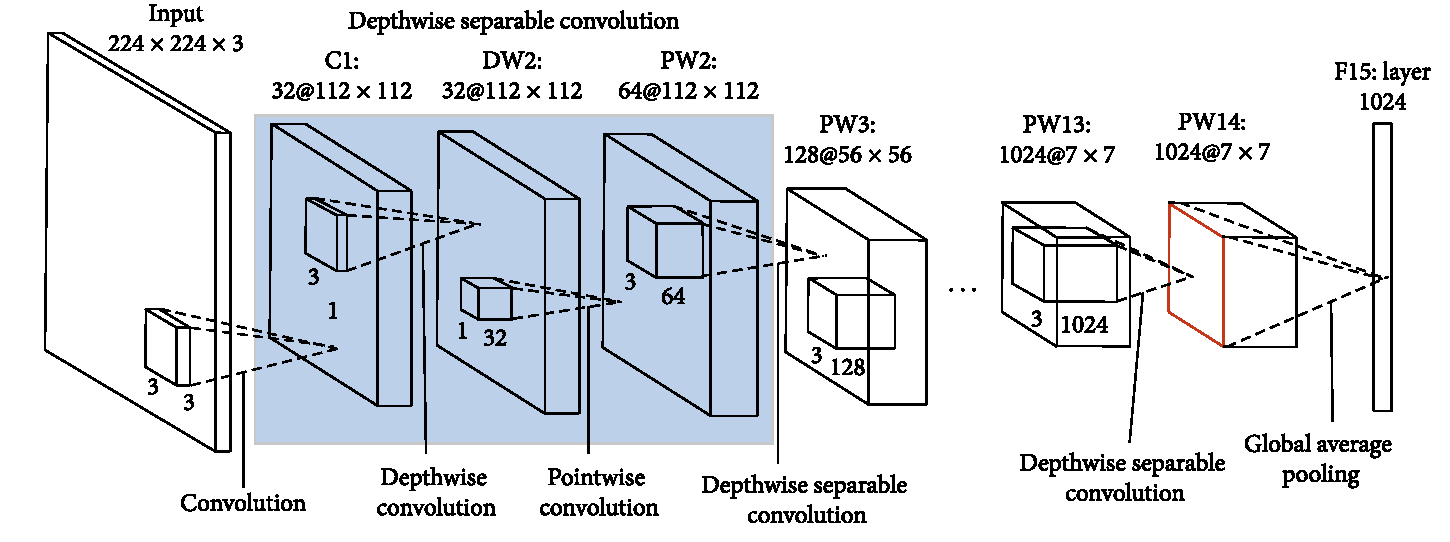
\includegraphics[width=\textwidth]{mobilenet}
            \caption{Architecture of \gls{mobilenet} Feature Extractor}
            \label{fig:mobilenet_arch}
        \end{figure}
        
    \section{Model and Network Architecture}
        For the purpose of localization of the detected potholes we used an existing object detector model named \acrfull{ssd}.
                
        \begin{figure}[h]
            \centering
            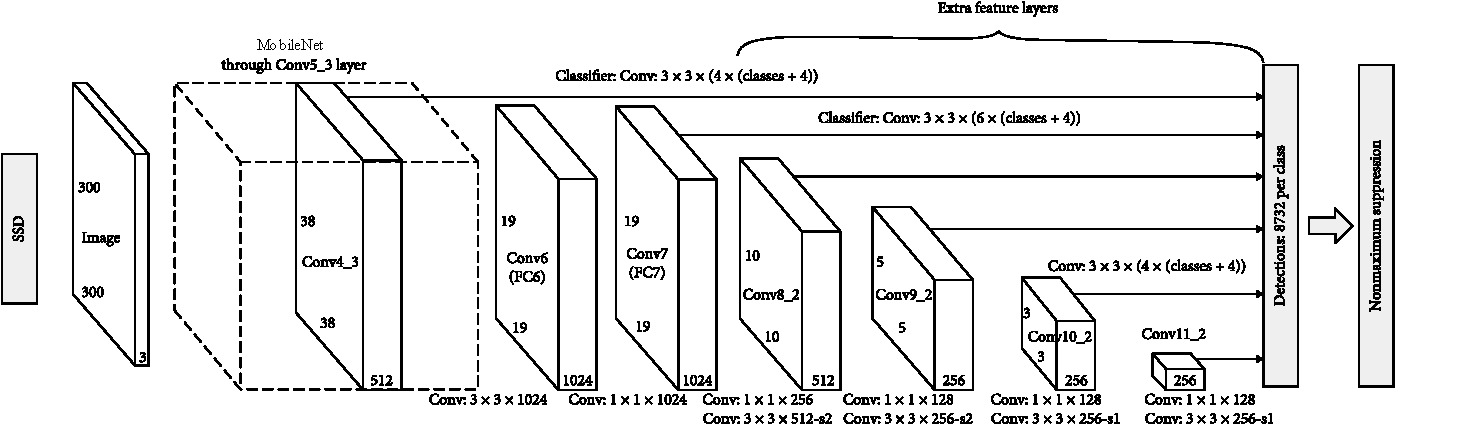
\includegraphics[width=\textwidth]{ssd}
            \caption{Architecture of Single Shot Multibox Detector}
            \label{fig:ssd_arch}
        \end{figure}
        
    \section{Activation Function}
        Our model uses the same ReLU activation function as the pre-trained model.
        \begin{figure}[h]
            \centering
            \begin{tikzpicture}
                \begin{axis}[axis x line*=bottom, axis y line*=left, ymax=6]
                    \addplot[mark=none] coordinates {
                        (-5, 0) (0, 0)
                        
                        (0, 0) (5, 5)
                    };
                \end{axis}
            \end{tikzpicture}
            \caption{Graphical View of the ReLU Activation Function}
            \label{fig:relu}
        \end{figure}
            
            
    \section{Training Method}
        We have trained our model on Google Cloud Platform, namely, Colaboratory by Google which provides an elegant runtime host for data-science experiments.  
            
        \subsection{Input Resizing}
            Our models takes input images of size $300\times 300\times 3$, meaning \acrshort{rgb} image having width of 300 pixels and height of 300 pixels. Therefore, it is required to preprocess any input image to convert it to a compatible shape for our model.
            We have resized the input image keeping the aspect ratio. If the input image is not square shaped, we stretched or contracted it until the longer side reaches 300 pixel. The remaining pixels then were padded by zero to make it $300\times 300$. 
            \begin{figure}[h]
                \centering
                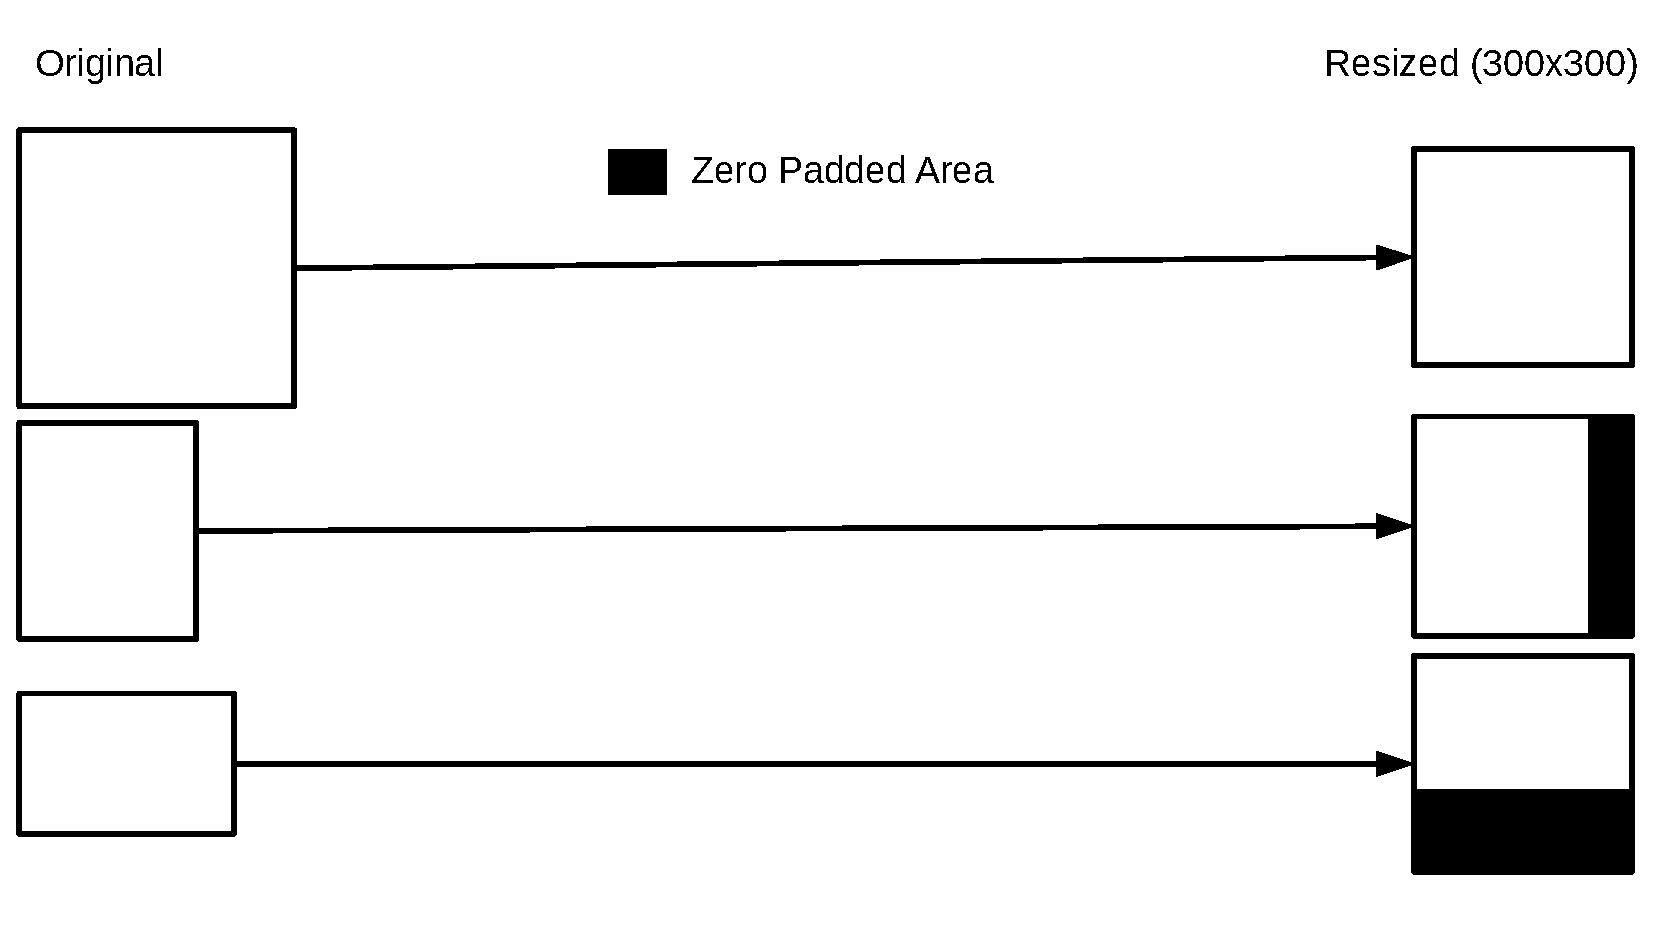
\includegraphics[width=\textwidth]{image-resizing}
                \caption{Input Resizing Mechanism}
                \label{fig:img_resize}
            \end{figure}          
            
        \subsection{Dataset Augmentation}
            Image augmentation is a technique to make the dataset larger in front of the model being trained when the actual dataset is small. Models trained with larger dataset usually performs better that that of trained with a small dataset.            
            We performed following augmentation operations on the input images at the time of training phase---
            
            \begin{itemize}
                \item Randomly crop a region of image.
                \item Randomly flip the image horizontally.
            \end{itemize}
            
        \subsection{Learning Rate}
            Learning rate defines how fast a model learns while training. Higher learning rate makes faster learning i.e. the model takes shorter time to complete training. But it has a bad side-effect--- the model may not converge to the optimum point, rather, it get stuck making back-and-forth weight updates. It may cause an oscillation to the gradient-descent path and never converge. Therefore, the learning rate must be selected in a way so that it is optimum for both convergence and training duration.
            \begin{figure}[h]
                \centering
                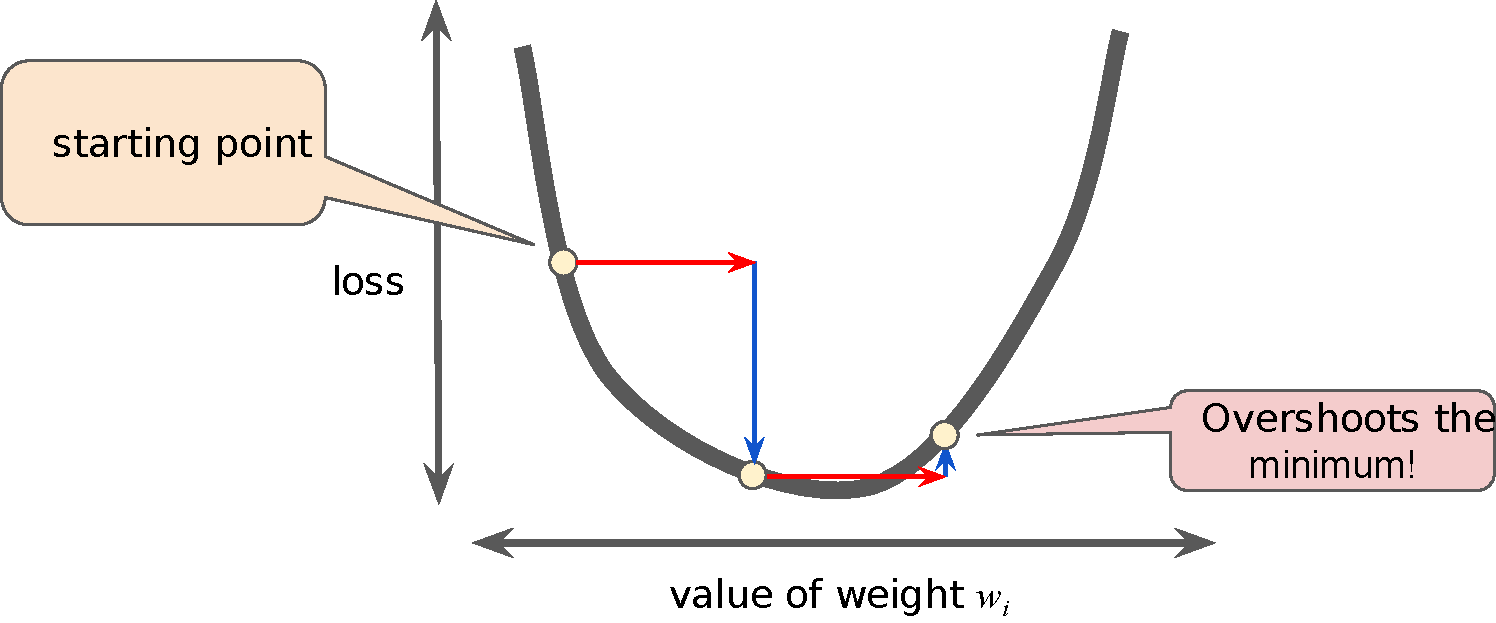
\includegraphics[width=\textwidth]{gradient-descent}
                \caption{Overshooting Caused by Higher Learning Rate}
                \label{fig:gradient_descent}
            \end{figure}
            
    \section{Validation Method}
        We have used a distinct validation dataset with respect to the training set for the purpose of the validation of our model.
        During this process, we used Microsoft \acrshort{coco} metric as standard.
        
        We built the model to not only detect the potholes but also localize them in the image or video frame. It yields the bounding boxes for each detected pothole. Bounding boxes cannot be treated as similar to those classification schemes where either of the classes are predicted to be. In classification, if the predicted class is similar to the actual class, it is treated as true-positive, otherwise false-negative. But in case of bounding-box detection, the output, model yields may not be exactly same as ground truth value but at the same time it may be inappropriate to consider as a false-negative prediction. As a solution to this problem, we take \acrfull{iou} measurement for performance evaluation.
            
        Here, taking account the \acrshort{iou} thresholds, \\
        $TP$ = Number of \acrlong{tp} Predictions \\
        $FP$ = Number of \acrlong{fp} Predictions \\
        $TN$ = Number of \acrlong{tn} Predictions \\
        $FN$ = Number of \acrlong{fn} Predictions
        
        \subsection{Intersection over Union}
            It is a method of measuring how accurately a model predicts and localizes an object in an image or video frame.
            
            We considered following \acrshort{iou} measures---
            \begin{enumerate}
            \item 50\% \acrshort{iou}
            \item 75\% \acrshort{iou}
            \item 50\%:5\%:95\% \acrshort{iou}
            \end{enumerate}
            An \acrshort{iou} of 50\%:5\%:95\% means a range where minimum value is 50\% and maximum is 95\% with an interval of 5\%. Therefore, it takes the average of the following 10 \acrshort{iou} thresholds--- 50\%, 55\%, 60\%, 65\%, 70\%, 75\%, 80\%, 85\%, 90\% and 95\%.
            
            \begin{figure}
                \centering
                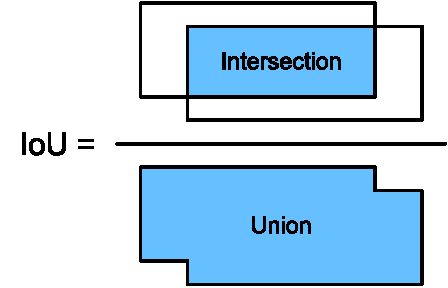
\includegraphics[width=\textwidth]{iou}
                \caption{IoU Calculation from Ground-Truth and Predicted Boxes}
                \label{fig:iou_calculation}
            \end{figure}

        \subsection{Precision Values}
            Precision shows how much the predictions are correct. That is, percentage of correct predictions among all the positive-predicted values.

            We considered and calculated precision for different  sizes of potholes as well as for different \acrshort{iou} thresholds---
            \begin{enumerate}
             \item mAP@50\% \acrshort{iou}
             \item mAP@75\% \acrshort{iou}
             \item mAP@50\%:5\%:95\% \acrshort{iou} for all sizes.
             \item mAP@50\%:5\%:95\% \acrshort{iou} for small sizes.
             \item mAP@50\%:5\%:95\% \acrshort{iou} for medium sizes.
             \item mAP@50\%:5\%:95\% \acrshort{iou} for large sizes.
            \end{enumerate}
            
            $$Precision = \frac{TP}{TP+FP}$$
            Average Precision is the area under precision-recall curve.
            $$AP = \int_{0}^{1}p(r) dr$$
        
        \subsection{Recall Values}
            We considered and calculated the recall values as another parameter of our model's performance evaluation.
            
            We considered and calculated recall for different  sizes of potholes as well as for different maximum detection levels---
            \begin{enumerate}
             \item AR@1 detection
             \item AR@10 detections
             \item AR@100 detections for all sizes
             \item AR@100 detection for small sizes
             \item AR@100 detection for medium sizes
             \item AR@100 detection for large sizes
            \end{enumerate}
            All of these recall values were calculated for 50\%:5\%:95\% \acrshort{iou} threshold.
            
            $$Recall = \frac{TP}{TP+FN}$$

                
    %%%%%%%%% END: Methodology %%%%%%%%%%
    

    
